\documentclass{beamer}
\usepackage[english]{babel}
\usepackage{geometry}
\usepackage[utf8]{inputenc}
\usepackage{colortbl}
\usepackage{listings}
\usepackage{adjustbox}
\usepackage{amsmath}
\usepackage{multirow}
\usepackage{tabularx}
\usepackage{tikz}
\usepackage[linewidth=1pt]{mdframed}
\usepackage[utf8]{inputenc}

\usetheme{Madrid}
% \usecolortheme{Copenhagen}
\usenavigationsymbolstemplate{} % no navigation buttons
\usecolortheme{beaver}

% \setbeamercolor{block title}{bg=red!30,fg=black}


\title{TCP/IP in hardware }
\subtitle{- using SME}
\author{Mark Jan Jacobi \& Jan Meznik}
\institute{University of Copenhagen}
\date{\today}


\begin{document}

\frame{\titlepage}

\section{Introduction}
\begin{frame}
  \frametitle{Background and Motivation}

  Dedicated hardware needs to transmit data in real time, but OS network 
  stacks are usually not enough!

  Dedicated Network cards are not perfect either:
  \begin{columns}

 \begin{column}{0.7\textwidth} 
  \begin{alertblock}{Weaknesses of network cards}
    \begin{itemize}
      \item Only basic programmability
      \item Incompatible APIs 
      \item Licensed VHDL code blobs
      \item Seldom swap-able
      \item \textbf{Price!}
    \end{itemize}
  \end{alertblock}
  \end{column}

  \begin{column}{0.3\textwidth}
    \begin{figure}
    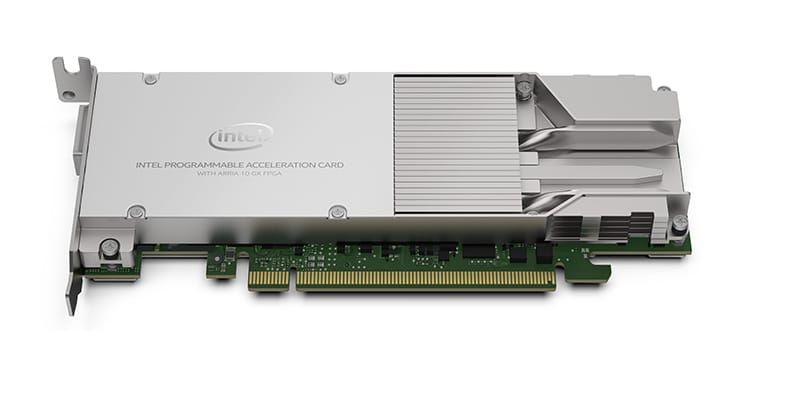
\includegraphics[scale=0.15,angle=270]{intel_fpga_nic.jpg}
    \caption{An Intel FPGA NIC}
    \end{figure}
  \end{column}

\end{columns}


\end{frame}
\begin{frame}
\begin{center}
  \textbf{A performant, efficient, and flexible network stack in FPGA!}
\end{center}

\begin{block}{How?    Using SME!}
  \begin{itemize}
    \item Easy \& intuitive hardware modelling
    \item Implicit clock
    \item Built-in simulation utilities 
    \item VHDL code generation 
    \item Verification by comparing VHDL signals with C\# simulation
  \end{itemize}
\end{block}

\end{frame}

\begin{frame}
  \frametitle{SME and FPGA}

  Skip this if SME has been covered
\end{frame}

\begin{frame}
  \frametitle{Internet Protocol Suite (TCP/IP)}
\begin{columns}

 \begin{column}{0.5\textwidth} 
  \begin{center}
  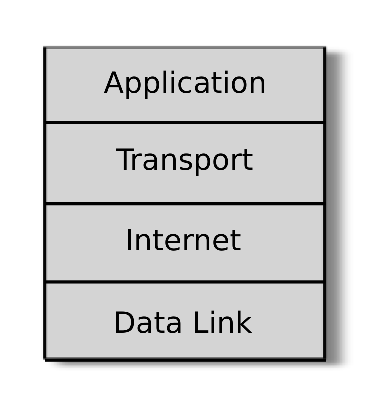
\includegraphics[scale=0.5]{tcpip_stack}
  \end{center}
  \end{column}

 \begin{column}{0.5\textwidth} 
 Some text
  
\end{column}
\end{columns}

\end{frame}



\section{Implementation}
\begin{frame}
  \frametitle{Architecture}
  \begin{center}
    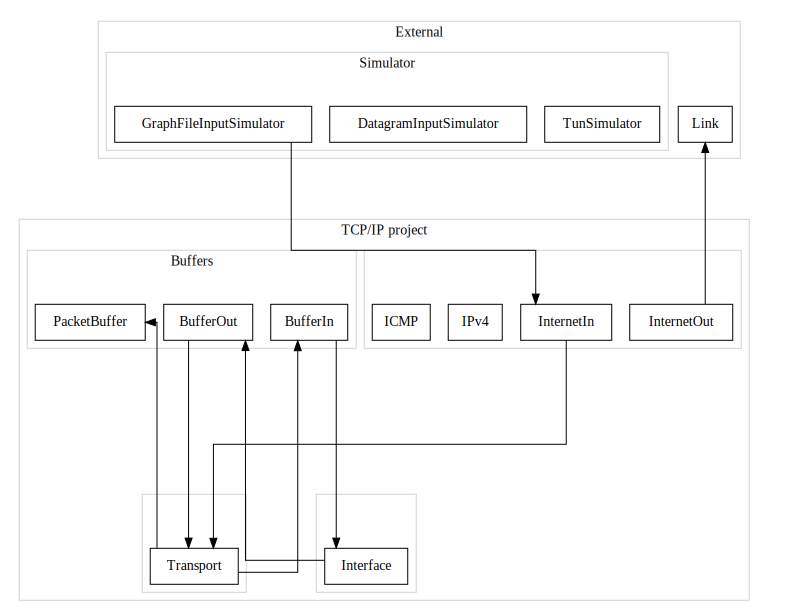
\includegraphics[scale=0.5]{graph}
  \end{center}
  

\end{frame}

\section{Challenges}
\begin{frame}
  \frametitle{Challenges}

\begin{itemize}
  \item Clock-delays
  \item Data de-multiplexing 
  \item Limited (fast) memory
  \item Information sharing is by design hard in SME
  \item Very limited programming utilities
\end{itemize}

\end{frame}

\section{Questions}
\begin{frame}
  \frametitle{Questions}
  \begin{center}
    ?
  \end{center}
\end{frame}


\end{document}



